\newcommand {\matr}[2]{\left[\begin{array}{#1}#2\end{array}\right]}
\newcommand{\E}{\mathbb{E}}
\newcommand{\tr}{\mathrm{tr}}
\newcommand{\x}{{\mathbf{x}}}
\renewcommand{\u}{{\mathbf{u}}}
\newcommand{\w}{{\mathbf{w}}}
\renewcommand{\r}{{\mathbf{r}}}


\chapter{Combining reinforcement learning and model based optimization}\label{ch:mpc}
\begin{center}
\textit{\textbf{RQ 3: How can AD domain knowledge and models be used to improve the action and state space for a RL agent?}}
\end{center}
\vspace{12pt}

\todo{as we see in previous chapter }

\section{MPC}
\todo{rewrite}
MPC is an optimization-based control technique where an Optimal Control Problem~(OCP) is repeatedly solved over a receding limited time horizon, starting from the current system state. In particular, for every time instance, a mathematical model of the controlled system is used to simulate the future states over a finite horizon, while a sequence of control inputs are selected and optimized given an objective cost function. The first element in the sequence of control inputs is then applied to the real system, and a new OCP with an updated state is solved at the next time instance.

\section{Approach, (Action space, options. MPC)}
MPC has a mixed integer problem, calculating the optimal path for all possible action is very computationally heavy. 
RL DQN. Only has discrete actions. Can not guarantee safety but is good at choosing actions with the best utility (value). 
The reward function takes in the predicted outcome of the model in the MPC and can penalize the choice of action. but if experience show that the outcome is better than the model, it can choose to take a bad action that would lead to a better total reward compared to only following a conservative model. 

\tommy{in this work we simulate three different intention agents, take way, give way and cautious agent.}
\begin{figure}[t!]
	\mbox{\parbox{\textwidth}{
	\centering
	% \vspace{0.3cm}
	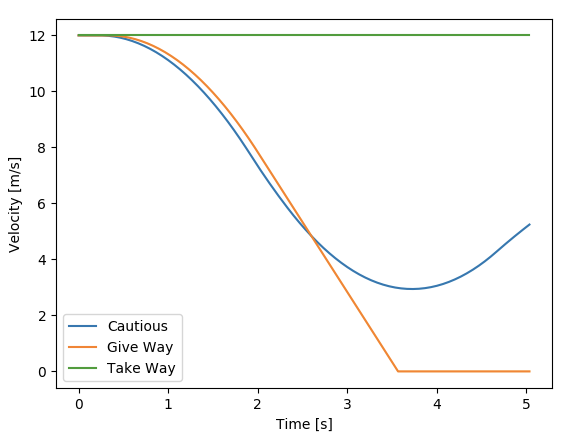
\includegraphics[width=0.7\columnwidth]{YourThesis/papers/mpc/figures/velocity_profiles_agents.png}
	}}
	\caption{Example of how velocity profile of the different intention agents can look like. All agents have the same starting velocity of $12$m/s and are approaching the same intersection}
	% \label{fig:intention_profiles}
	% \vspace{-0.3cm}
\end{figure}\
\todo{reward function}
added Q masking.
Q-masking reduce the search space, in this work we showed it for unavailable actions but could be extended to actions limited by the precautionary safety module. 
By combining the having the mpc cost as a negative rewward the \gls{dqn} can balance the control cost with the high level goal of reaching the goal and even choose an action that is on average good on a high level but may not seem that way to the \gls{mpc}.

Given the state representation, the dynamics of the vehicle is then modeled using a  triple integrator with jerk as control input.

\tommy{mpc cost function}
The objective of the agent is to safely track a reference, e.g. follow a path with a target speed, acceleration, and jerk profile, while driving comfortably and satisfying constraints that arise from physical limitations and other road users, e.g. not colliding in intersections with crossing vehicles. Hence, we formulate  the  problem as a finite horizon, constrained optimal control problem
\begin{subequations}
	\label{eq:mpc2}
	\begin{align}
	J = \min_{\bar\x,\bar\u} & \sum_{k=0}^{N-1}% \varphi_n(x_n,u_n) + \varphi_N(x_N)\\
	\matr{c}{\bar\x_k - \r_k^\x \\ \bar\u_k - \r_k^\u}^\top \matr{cc}{Q &S^\top\\S & R} \matr{c}{\bar\x_k - \r_k^\x \\ \bar\u_k - \r_k^\u} \\
	&\qquad + \matr{c}{\bar\x_N - \r_N^\x}^\top P \matr{c}{\bar\x_N - \r_N^\x}\nonumber\\
	&\text{s.t.}\ \ \, \bar\x_0 = \hat{\x}_0, \label{eq:mpcState2}\\
	&\qquad{}\bar\x_{k+1} = A\bar\x_{k}+B\bar\u_{k},\label{eq:mpcDynamics2}\\
	&\qquad{}h(\bar\x_k,\bar\u_k,\bar{\mathbf{o}}_k,a_k) \leq{} 0, \label{eq:mpcInequality2}
	\end{align}
\end{subequations}
where $k$ is  the prediction time index, $N$ is the prediction horizon, $Q$, $R$, and $S$ are the stage costs, $P$ is the terminal cost, $\bar\x_k$ and $ \bar\u_k$ are the predicted state and control inputs, $\r^\x_k$ and $\r^\u_k$ are the state and control input references, $\bar{\mathbf{o}}_k$ denotes the predicted state of vehicles in the environment which need to be avoided, and $a$ is the action from the high-level decision maker. Constraint \eqref{eq:mpcState} enforces that the prediction starts  at the current state estimate $\hat\x_0$, \eqref{eq:mpcDynamics} enforces the system dynamics, and \eqref{eq:mpcInequality} enforces constraints on the states, control inputs, and obstacle avoidance.

The reference points, $\r^\x_k$, $\r^\u_k$ are assumed to be set-points of a constant velocity trajectory, e.g. following the legal speed-limit on the road. Therefore, we set the velocity reference according to the driving limit, and the acceleration and jerk to zero.


% \tommy{Obstacle prediction}
% In order for the vehicle planner in \eqref{eq:mpc} to be able to properly avoid collisions, it is necessary to provide information about the surrounding vehicles in the environment. Therefore, similarly to \cite{batkovic2019}, we assume that a sensor system provides information about the environment, and that there exists a prediction layer which generates future motions of other vehicles in the environment. The accuracy of the prediction layer will heavily affect the performance of the planner, hence, it is necessary to have computationally inexpensive and accurate prediction methods.

% In this paper, for simplicity the future motion of other agents is estimated by a constant velocity prediction model. The motion is predicted at every time instant for prediction times $k\in[0,N]$, and is used to form the collision avoidance constraints, which we describe in the next section. Even though more accurate prediction methods do exist, e.g. \cite{lefevre2014survey,batkovic2018}, we use this simple model to show the potential of the overall framework.

% \tommy{Collision avoidance}
% % \begin{figure}[t]
% % 	\centering
% % 	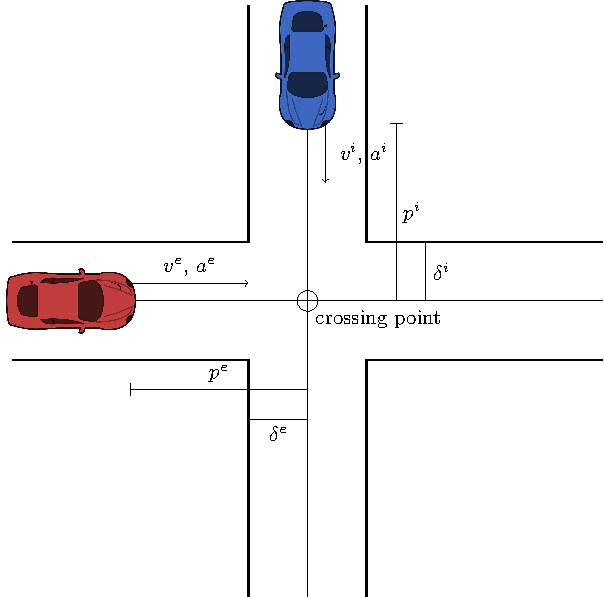
\includegraphics[width=0.6\columnwidth]{figures/figures-observations.pdf}
% % 	\caption{Observations of a scenario}
% % 	\label{fig:observations2}
% % \end{figure}\
% We denote a vehicle $j$ with the following notation $\x^j:=[p^j\, v^j\, a^j]^\top$, and an associated crossing point at position $p^{\mathrm{cross},j}$ in its own vehicle frame, which translated into the ego-vehicle frame is denoted as $p^{\mathrm{cross},j}_\mathrm{ego}$. With a predefined road topology, we assume that the vehicles will travel along the assigned paths, and that collisions may only occur at the crossing points $p^{\mathrm{cross},j}$ between an obstacle and the ego vehicle. Hence, for collision avoidance, we use the predictions of the future obstacle states $\bar\x^j_k$ for times $k\in[0,N]$, provided by a prediction layer outside of the MPC framework. Given the obstacle measurements, the prediction layer will generate future states throughout the prediction horizon. With this information, it is possible to identify the time slots when an obstacle will enter the intersection.

% Whenever an obstacle $j$ is predicted to be within a threshold of $p^{\mathrm{cross},j}$, e.g. the width of the intersecting area, the ego vehicle faces a constraint of the following form
% \begin{gather*}
% \bar{p}_k^\mathrm{e} \geq{} p^{\mathrm{cross},j}_\mathrm{ego} + \Delta,\quad\underline{p}_k^\mathrm{e} \leq{} p^{\mathrm{cross},j}_\mathrm{ego} - \Delta,
% \end{gather*}
% where $\Delta$ ensures sufficient padding from the crossing point that does not cause a collision. The choice of $\Delta$ must be at least such that $p_k$ together with the dimensions of the ego-vehicle does not overlap with the intersecting area.

% \tommy{Take way and give way constraint}
% Since the constraints from the surrounding obstacles become non-convex, we rely on the high-level policy maker to decide through action $a$ how to construct the constraint \eqref{eq:mpcInequality} for Problem \eqref{eq:mpc}. The take-way action implies that the ego-vehicle drives first through the intersection, i.e., it needs to pass the intersection before all other obstacles. This implies that for any vehicle $j$ that reaches the intersection during prediction times $k\in[0,N]$, the generated constraint needs to lower bound the state $p_k$ according to
% \begin{equation}
% \max_{j}p^{\mathrm{cross},j}+\Delta \leq{}p_k^\mathrm{e}.
% \end{equation}
% Similarly, if the action is to give way, then the position needs to be upper bounded by the closest intersection point so that
% \begin{equation}
% p_k^\mathrm{e} \leq{} \min_{j}p^{\mathrm{cross},j}_\mathrm{ego}-\Delta,
% \end{equation} 
% for all times $k$ that the obstacle is predicted to be in the intersection.

% \tommy{Following an obstacle}
% For any action $a$ that results in the following of an obstacle $j$, the ego-vehicle position is upper bounded by $p^\mathrm{e}_k \leq{} p^\mathrm{cross,j}_\mathrm{ego}$. We construct constraints for obstacles $i\neq{}j$ according to
% \begin{itemize}
% 	\item if $p^\mathrm{cross,i}<{}p^\mathrm{cross,j}$ then $p^\mathrm{cross,i}+\Delta\leq{}p_k^\mathrm{e}$, which implies that the ego-vehicle should drive ahead of all obstacles $i$ that are approaching the intersection;
% 	\item if $p^\mathrm{cross,i}>{}p^\mathrm{cross,j}$ then $p_k^\mathrm{e}\leq{}p^\mathrm{cross,i}-\Delta$, which implies that the ego-vehicle should wait to pass obstacle $j$ and other obstacles $i$;
% 	\item if $p^{\mathrm{cross,i}}=p^{\mathrm{cross},j}$ then the constraints generated for obstacle $i$ becomes an upper or lower  bound depending on if obstacle $i$ is ahead or behind the obstacle $j$ into the intersection.
% \end{itemize}


\section{Simulated experiments}
We show the difference in a multi crossing scenario where the MPC can plan a path for both intersections while our previous DQN only handles one at a time. 

\begin{figure}[t]
	\mbox{\parbox{\textwidth}{
	\centering
	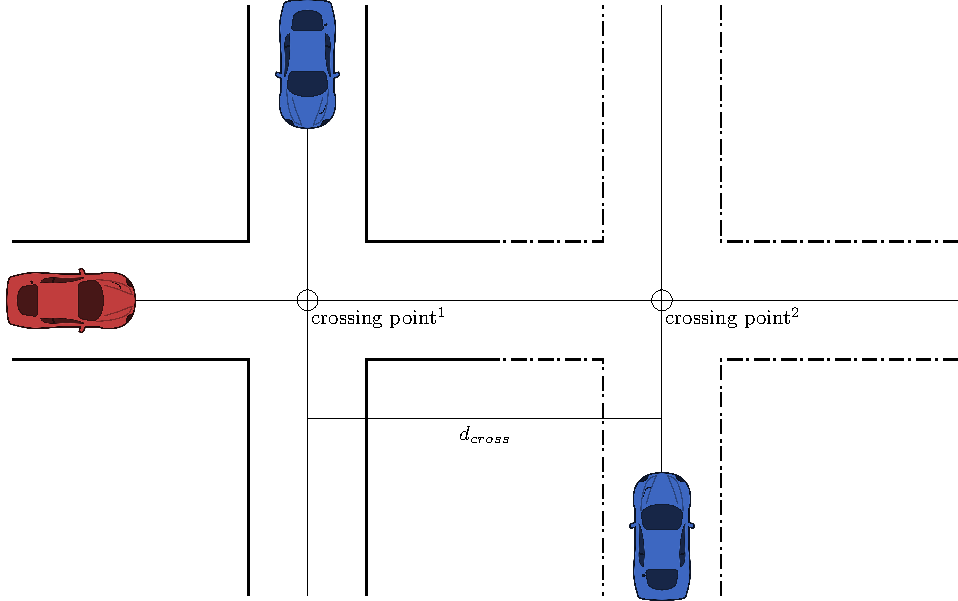
\includegraphics[width=.95\columnwidth]{YourThesis/papers/mpc/figures/figures-scenarios.pdf}
	}}
	\caption{Illustration of a intersection scenario, where the solid line is a single crossing and together with the dashed line creates a double crossing.}
	% \label{fig:scenario}
\end{figure}

\section{Results and discussion}

% \begin{figure}[t!]
	% \mbox{\parbox{\textwidth}{
% 	\centering
% 	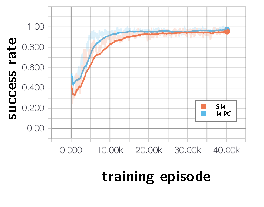
\includegraphics[width=\columnwidth]{YourThesis/papers/mpc/figures/figures-successrate.pdf}
% }}
% 	\caption{Average MPC and SM success rate for a single corssing after evaluating the policy 300 episodes.}
% 	\label{fig:result1}
% \end{figure}

% \begin{figure}[t!]
% 	\centering
% 	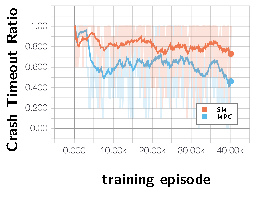
\includegraphics[width=\columnwidth]{YourThesis/papers/mpc/figures/figures-crashratio.pdf}
% 	\vspace{-4em}
% 	\caption{Average MPC and SM crash to timeout ratio for a single crossing after evaluating the policy in 300 episodes. A CTR of $0$ means that all failures are timeouts, while a CTR of $1$ means that all failures are collisions.}
% 	\label{fig:result2}
% \end{figure}

\begin{table}[t!]
	\mbox{\parbox{\textwidth}{
	\centering
	\begin{tabular}{ |p{1,6cm}||p{1,2cm}|p{1,2cm}|p{1,2cm}|p{1,2cm}|}
	\hline
	Controller &\multicolumn{2}{|c|}{Success Rate}
	&\multicolumn{2}{|c|}{Timeout Ratio}\\
	\hline
	 & Single & Double & Single & Double\\
	\hline
	SM & $96.1\%$ & $90.9\%$ & $72\%$ & $93\%$\\
	MPC & $97.3\%$ & $95.2\%$ & $45\%$ & $76\%$\\
	\hline
	\end{tabular}
	}}
	\caption{Average success rates and collision to timeout rates.}% across single and double crossings.}   

% \label{tab:successrate}
\end{table}

synergies between mpc and dqn